
\documentclass[letterpaper, reqno,11pt]{article}
\usepackage[margin=1.0in]{geometry}
\usepackage{color,latexsym,amsmath,amssymb}
\usepackage{fancyhdr}
\usepackage{amsthm}
\usepackage[linesnumbered,lined,boxed,commentsnumbered,noend,noline]{algorithm2e}
\usepackage{dsfont}
\usepackage{graphicx}
\usepackage{hyperref}
\usepackage{bbm}
\usepackage[inline]{enumitem}
\usepackage[numbers]{natbib}
\usepackage{framed}
\usepackage{titling}
\usepackage{subcaption}
\usepackage[dvipsnames]{xcolor}
\usepackage{tikz}

\tikzset{invclip/.style={clip,insert path={{[reset cm]
  (-16383.99999pt,-16383.99999pt) rectangle (16383.99999pt,16383.99999pt)}}}}

\allowdisplaybreaks

\newcommand{\RR}{\mathbb{R}}
\newcommand{\CC}{\mathbb{C}}
\newcommand{\ZZ}{\mathbb{Z}}
\newcommand{\QQ}{\mathbb{Q}}
\newcommand{\NN}{\mathbb{N}}
\newcommand{\FF}{\mathbb{F}}
\newcommand{\PP}{\mathbb{P}}
\newcommand{\EE}{\mathbb{E}}
\newcommand{\LL}{\mathbb{L}}
\newcommand{\TT}{\mathbb{T}}
\newcommand{\GI}{\textrm{GI}}
\newcommand{\coGI}{\overline{\textrm{GI}}}
\DeclareMathOperator{\conv}{conv}
\DeclareMathOperator{\charcone}{char.cone}
\DeclareMathOperator{\STAB}{STAB}
\DeclareMathOperator{\Down}{Down}
\DeclareMathOperator{\lca}{lca}
\DeclareMathOperator{\ex}{ex}
\DeclareMathOperator{\Span}{span}
\DeclareMathOperator{\T}{T}
\DeclareMathOperator{\F}{F}
\DeclareMathOperator{\shP}{\# P}
\DeclareMathOperator{\shSAT}{\# SAT}
\DeclareMathOperator{\shDNF}{\# DNF}
\DeclareMathOperator{\DNF}{DNF}
\DeclareMathOperator{\Poly}{P}
\DeclareMathOperator{\CNF}{CNF}
\DeclareMathOperator{\SAT}{SAT}
\DeclareMathOperator{\BPP}{BPP}
\DeclareMathOperator{\poly}{poly}
\DeclareMathOperator{\RP}{RP}
\DeclareMathOperator{\EXP}{EXP}
\DeclareMathOperator{\DTIME}{DTIME}
\DeclareMathOperator{\NP}{NP}
\DeclareMathOperator{\MCprime}{MC'}
\DeclareMathOperator{\Var}{Var}
\DeclareMathOperator{\IP}{IP}
\DeclareMathOperator{\PSPACE}{PSPACE}
\DeclareMathOperator{\lollipop}{lollipop}
\newcommand\mycommfont[1]{\ttfamily\textcolor{blue}{#1}}
\SetCommentSty{mycommfont}
\begin{document}
\pagenumbering{arabic}
\title{Lectures on Random Walks}
\author{Yuchong Pan}
\date{\today}
\newtheorem{theorem}{Theorem}
\newtheorem{lemma}[theorem]{Lemma}
\newtheorem{proposition}[theorem]{Proposition}
\newtheorem{corollary}[theorem]{Corollary}
\newtheorem{fact}[theorem]{Fact}
\newtheorem{problem}[theorem]{Problem}
\newtheorem{claim}{Claim}
\newtheorem{exercise}{Exercise}
\theoremstyle{definition}
\newtheorem{definition}[theorem]{Definition}
%\maketitle
%

\begin{framed}
\noindent{\bf 6.842 Randomness and Computation} \hfill \thedate
\begin{center}
\Large{\thetitle}
\end{center}
\noindent{\em Lecturer: Ronitt Rubinfield} \hfill {\em Scribe: \theauthor}
\end{framed}

\section{Definitions}

\begin{definition}
  Let $\Omega$ be a set of states (throughout this note, $\Omega$ is finite). A sequence of random walks $X_0, X_1, \ldots \in \Omega$ is a \emph{Markov chain} if it satisfies the \emph{Markovian property}, i.e., for each $t \in \NN$ and for all $x_1, \ldots, x_t, y \in \Omega$,
  $$ \PP\left[X_{t + 1} \;\middle|\; X_1 = x_1, \ldots, X_t = x_t\right] = \PP\left[X_{t + 1} = y \;\middle|\; X_t = x_t\right]. $$
  WLOG, we assume that transitions are independent of time. For $x, y \in \Omega$, let
  $$ P(x, y) = \PP\left[X_{t + 1} = y \;\middle|\; X_t = x\right]. $$
  Interpreted as a matrix, $P$ is called the \emph{transition matrix} of the Markov chain. We can also interpret the transition matrix $P$ as a weighted directed graph with vertex set $\Omega$ such that the weight on $(i, j) \in \Omega^2$ equals $P(i, j)$.
\end{definition}

A random walk on a directed graph is a special case of Markov chains.

\begin{definition}
  A \emph{random walk} on a directed graph $G = (V, E)$ is a sequence $S_1, S_2, \ldots \in V$ such that $S_{t + 1}$ is picked uniformly in $N^+(S_t)$, i.e., the transition matrix $P$ is defined so that for $x, y \in V$,
  $$ P(x, y) = \left\{
    \begin{array}{ll}
      \frac{1}{d^+(x)}, & \text{if $(x, y) \in E$}, \\
      0, & \text{otherwise}.
    \end{array}
  \right. $$
\end{definition}

\begin{definition}
  An $n \times n$ matrix $P$ is called a \emph{stochastic matrix} if for all $i \in [n]$,
  $$ \sum_{i = 1}^n P(i, j) = 1. $$
\end{definition}

For each $t \in \NN$, let $P_t(x, y)$ ve the transition probability from $x$ to $y$ for $t$ steps. Then for all $x, y \in \Omega$ and $t \in \NN$,
$$ P^t(x, y) = \left\{
  \begin{array}{ll}
    P(x, y), & \text{if $t = 1$}, \\
    \sum_{z \in \Omega} P(x, z) P^{t - 1}(z, y) & \text{if $t > 1$}.
  \end{array}
\right. $$
Interpreted as matrix multiplication, for each $t \in \NN$ with $t > 1$,
$$ P^t = P \cdot P^{t - 1}. $$
Let $\Pi^{(0)} = (\Pi_1^{(0)}, \ldots, \Pi_n^{(0)})$ be the initial distribution, where $\Pi_i^{(0)}$ is the probability of starting at vertex $i$ for each $i \in [n]$.\footnote{WLOG, we assume $\Omega = [n]$.} Let $\Pi^{(t)}$ be the distribution after $t$ steps for each $t \in \NN$. For each $t \in \NN$,
$$ \Pi^{(t)} = \Pi^{(0)} P^t. $$

\begin{definition}
  A distribution $\Pi^*$ is called a \emph{stationary distribution} of a Markov chain with state set $\Omega$ and transition matrix $P$ if for all $x \in \Omega$,
  $$ \Pi^*(x) = \sum_{y \in \Omega} \Pi^*(y) P(y, x). $$
\end{definition}

\begin{definition}
  A Markov chain with state set $\Omega$ and transition matrix $P$ is said to be \emph{irreducible} if for all $x, y \in \Omega$, there exists $t \in \NN$ such that $P^t(x, y) > 0$.
\end{definition}

\begin{definition}
  A Markov chain with state set $\Omega$ and transition matrix $P$ is said to be \emph{aperiodic} if for all $x \in \Omega$,
  $$ \gcd\left\{ t \in \NN : p^t(x, x) > 0 ]\right\} = 1. $$
\end{definition}

\begin{definition}
  A Markov chain with state set $\Omega$ and transition matrix $P$ is said to be \emph{ergodic} if there exists $t^* \in \NN$ such that for all $t \in \NN$ with $t > t^*$ and for all $x, y \in \Omega$, we have $P^t(x, y) > 0$.
\end{definition}

\begin{theorem}
  Every ergodic Markov chain has a unique stationary distribution.
\end{theorem}

In the special case of a random walk on an undirected graph $G = (V, E)$, the stationary distribution $\Pi^* = (\Pi_1^*, \ldots, \Pi_n^*)$ is given by $\Pi_i^* = d(i)/(2|E|)$ for all $i \in [n]$. Therefore, for a random walk on a $d$-regular graph or on a directed graph with each in-degree and each out-degree equal to $d$, the stationary distribution is uniform; this is not true in general directed graphs.

\section{Hitting Time, Cover Time and Commute Time}

\begin{definition}
  Consider a random walk on a graph $G = (V, E)$. For $x, y \in V$, the \emph{hitting time} $H_{x, y}$ is defined to be the expected number of steps to go from $x$ to $y$. For each $x \in V$, we call $H_{x, x}$ the \emph{recurrence time} for $x$.
\end{definition}

\begin{theorem}
  Consider a random walk on a graph $G = (V, E)$ with stationary distribution $\Pi^*$. For each $x \in V$,
  $$ h_{x, x} = \frac{1}{\Pi_*(x)}. $$
\end{theorem}

\begin{proof}[Proof sketch]
  Consider a very long walk. Then a $\Pi^*(x)$ fraction of the positions are $x$. Then the average gap between the occurrences of $x$ is $h_{x, x} = \Pi^*(x)^{-1}$.
\end{proof}

\begin{definition}
  Consider a random walk on a graph $G = (V, E)$. For $u \in V$, the \emph{cover time} $C_u(G)$ is defined to be the expected steps from $u$ to visit all states in $\Omega$. Define $C(G) = \max_{u \in V} C_u(G)$.
\end{definition}

Following are several examples of the cover time:
\begin{itemize}[itemsep=0pt]
  \item $C(K_n) = \Theta(n \log n)$, where $K_n$ is the complete graph on $n$ vertices with a self-loop at each vertex. This can be proved by a coupon collector argument.
  \item $C(L_n) = \Theta(n^2)$, where $L_n$ is the $n$-vertex line graph with a self-loop at each vertex.
  \item $C(\lollipop_n) = \Theta(n^3)$, where $\lollipop_n$ is an $n$-vertex lollipop vertex formed by $L_{n/2}$ and $K_{n/2}$ joined at a vertex. This is illustrated in Figure \ref{fig:lollipop}.
  
  \begin{figure}[h]
    \centering
    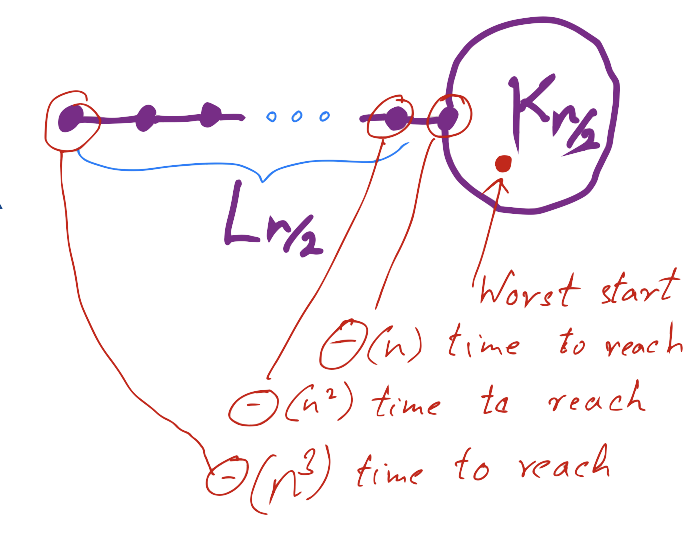
\includegraphics[width=.6\textwidth]{figures/lollipop.png}
    \caption{A lollipop graph $\lollipop_n$ and its cover time.}
    \label{fig:lollipop}
  \end{figure}
\end{itemize}

\begin{theorem} \label{thm:cover}
  Let $G$ be an undirected graph. Then\footnote{When the context is clear, we denote $m = |E|$ in a graph $G = (V, E)$.}
  $$ C(G) \leq O(mn). $$
\end{theorem}

\begin{definition}
  Consider a random walk on a graph $G = (V, E)$. For $x, y \in V$, the \emph{commute time} $C_{x, y} = C_{x, y}(G)$ is defined to be the expected number of steps for the random walk to start at $x$, hit $y$ and return to $x$.
\end{definition}

\begin{proposition}
  For $x, y \in V$,
  $$ C_{x, y} = h_{x, y} + h_{y, x}. $$
\end{proposition}

\begin{proof}
  This is due to linearity of expectation.
\end{proof}

\begin{lemma}
  Consider a random walk on a connected undirected graph $G = (V, E)$. For each $(x, y) \in E$,
  $$ C_{x, y} \leq O(m). $$
\end{lemma}

\begin{proof}
  Construct a graph $G'$ by adding a self-loop at each vertex with probability $1/2$. Let $x, y \in V$. We claim that $C_{x, y}(G') = 2C_{x, y}(G)$. To see this, for each path from $x$ to $y$ in $G'$, removing the self-loops in the path gives a path in $G$, and the expected fraction of self-loops in the path is $1/2$. Then $G'$ is ergodic. This implies that there exists a unique stationary distribution $\Pi^*$.

  Consider a walk $u_1, u_2, \ldots$, where $u_i \in V$ and $(u_i, u_{i + 1}) \in E$ for each $i \in \NN$. We look for commutes of the form
  $$ x \to y \to \ldots \to x \to y. $$
  For each $i \in \NN$,
  $$ \PP\left[u_i = x, u_{i + 1} = y\right] = \PP\left[u_i = x\right] \cdot \PP\left[u_{i + 1} = y \;\middle|\; u_i = x\right] = \frac{d(x)}{2m} \cdot \frac{1}{d(x)} = \frac{1}{2m}. $$
  Therefore, the expected fraction of $x \to y$ equals $1/(2m)$. This implies that the expected gap between the $(x \to y)$'s equals $2m$. This proves that $C_{x, y}(G) = O(m)$.
\end{proof}

\begin{proof}[Proof of Theorem \ref{thm:cover}]
  Let $T$ be a spanning tree of $G$. Let $(v_0, v_1, \ldots, v_{2n - 2})$ be a DFS traversal of $T$. For instance, $(1, 2, 3, 2, 4, 2, 1, 5, 1)$ is a DFS traversal of the tree given in Figure \ref{fig:dfs}. Then
  $$ C(G) \leq \sum_{i = 0}^{2n - 3} h_{v_i, v_{i + 1}} = \sum_{(x, y) \in E(T)} C_{x, y} \leq (n - 1) \cdot O(m) = O(mn). $$
  This completes the proof.

  \begin{figure}[h]
    \centering
    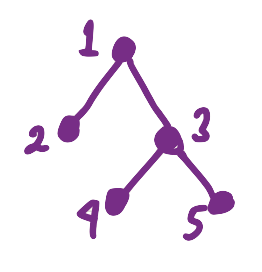
\includegraphics[width=.3\textwidth]{figures/dfs.png}
    \caption{$(1, 2, 3, 2, 4, 2, 1, 5, 1)$ is a DFS traversal of the tree in the figure.}
    \label{fig:dfs}
  \end{figure}
\end{proof}

\end{document}
